\subsection{Studies of data from {\rem}}
\protect\label{section:rem}

In this section is analysed observational data from the
REM (Rapid Eye Mount) telescope and camera equipment in La Silla, Chile, as
operated by the Red Dots Project. The observatory at La Silla was initially set up in 2003
\citep{antonelli05} consisting of the the REMIR near-infrared camera and the
visible light camera, ROSS. Light from the 60cm telescope is split at 1 $\mu$m into two beams
by a dichroic element. The light with wavelength greater than this passes to the
REMIR near-infrared camera and the smaller wavelengths to the ROSS camera.
The performance of the ROSS camera was not satisfactory and in 2015 it
was replaced by the ROSS2 camera system, described in outline at
\citet{reminaf7} and in more detail in \citet{molinari14}.

The work for this paper has focused on the ROSS2 visible light data. The same
patch of sky is viewed via 4 filters on this part of the telescope with exactly
the same exposure, in addition to 3 filters, combined with various dither
patterns by the REMIR telescope.

The REM telescope has been set up to take a series of automatic
observations of patches of sky on a nearly nightly basis. The main concern of
the Red Dots Project is of 3 {\rdwarf} stars, including {\prox} and {\bstar} as
well as \ross, but the REM observatory is concurrently used for other projects,
for example \citet{giannini18}.

The first observations of {\rdwarf} stars took place in mid-2017. All
observations ceased on March 2020 due to the Coronavirus pandemic but were
restarted in October 2020 and have continued up until April 2022. Between 6
August 2017 and 23 March 2022, 48,925 images including {\ross} were taken at
once, with a variety of filters. \texttt{g'}, \texttt{r'}, \texttt{i'} and
\texttt{z'}, hereinafter referred to as \texttt{g}, \texttt{r}, \texttt{i} and
\texttt{z} respectively.

\subsubsection{{\rem} observations of \ross}
\protect\label{section:remross}

Of the REM observations of \ross, 23,236 were taken using visible light filters
5,809 were taken using the \texttt{r} filter and after excluding 412 blank,
excessively noisy or otherwise unusable images, 5,297 were used, taken between 6
August 2017 and 23 March 2022.

Along with the images, a series of bias and flat files were collected daily and
these were used to create master bias and flat files.\footnote{Master monthly
daily flat and bias files were also created by the Red Dots Project, but these
were rejected for a variety of reasons, the most important being that the bias
files, after subtraction, rendered the pixel values negative in places both in
the image files and also in the daily flat files.}

The method of calibration used was to take the mean flux for each reference
star and then for each image and using each reference star within the image
construct a linear regression line. There are typically over 100 reference
stars available in each image, however the subset of reference stars out of the
set of over 600 possible ones for {\ross} is different for each frame as the
orientation of telescope and the position of {\ross} within the frame varies, or
objects are obliterated by cosmics and other issues.

The linear regression technique proved to have a very high correlation of
95\% or more in most cases. It was then possible to map the flux from {\ross}
back to a deviation from the mean and factors such as airmass, moon phase and so
forth consistently eliminated.

After calibration, the flux was calculated for the various observations from each
of the usable frames as shown in Fig \ref{fig:rossallcurve}.

\begin{figure}[!htbp]
\begin{center}
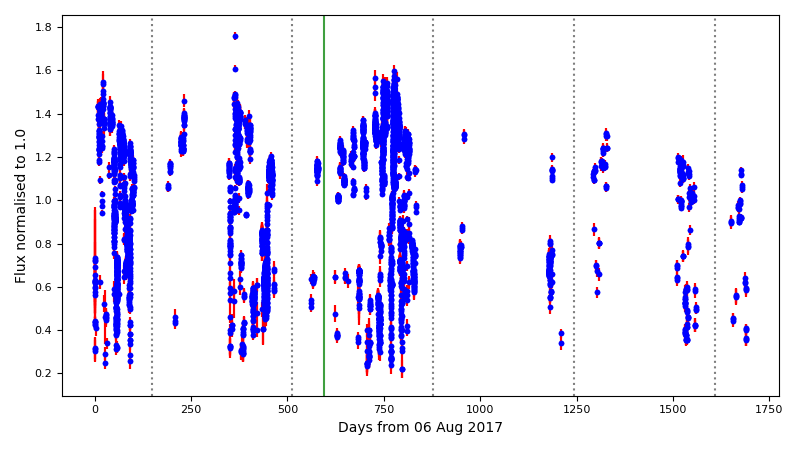
\includegraphics[scale=0.40]{REM/images/remrossallcurve.png} \\
\vspace{-.5cm}
\end{center}   
\caption{This shows the total flux after calibration from {\ross}
found in all acceptable images in {\rem}
observations, normalised so that the mean is 1.0. There was a change in
configuration in late March 2019, indicated by the sold vertical green line, but
this occurred 595 days from the start and thus does
not account for any of the shape of the plot
shown. The dotted vertical lines indicate the
start of the years 2018 through to 2022.}\protect\label{fig:rossallcurve}
\end{figure}

It proved hard to construct a clear periodogram from this data due to the
significant intervals between observations. Also only 4 or 5 observations are done in one
night, sometimes days apart, and this is far too small for any meaningful
results to be obtained. The observations are typically taken nightly at
the same time each night and this introduces a cycle close to the
rotation period. Attempts to produce periodograms from all the data yielded
numerous peaks, very densely packed but samples of observations taken much
closer together were more acceptable. In Fig.
\ref{fig:rossallpgram} is shown the portion between 2 and 5 days for the observations taken during 2022.

\begin{figure}[!htbp]
\begin{center}
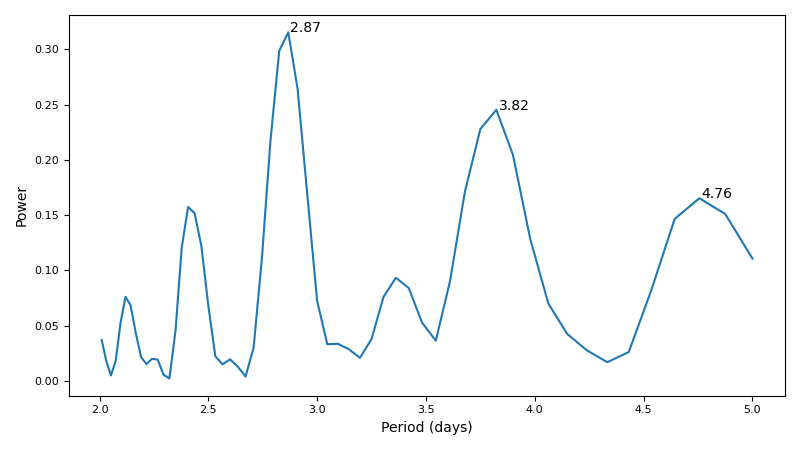
\includegraphics[scale=0.40]{REM/images/rem2022pgram.png} \\
\vspace{-.5cm}
\end{center}   
\caption{This shows part of the periodogram derived from the the data shown in
Fig. \ref{fig:rossallcurve} pertaining to 2022 (up
to 23 March), restricting the display to 2 to 5 days.}\protect\label{fig:rossallpgram}
\end{figure}

\IfThesis{
\subsubsection{Improving the {\rem} observation calibration}
\protect\label{section:remrosscalib}

The above flux from {\ross} was just on the flux alone, but did not take into
account other stars and factors such as air mass, weather and other influences
on the flux. By identifying the other stars in the object, discarding variable
and irregularly-shaped objects, such as binary or objects closer together than
the telescope resolution (approximately 0.6 arc second per pixel) could separate,
the remaining objects could be ordered, in descending brightness and also by
frequency of occurrence in the images, (as some of the possible reference stars
were outside the edges of the image for some frames).

A periodogram was produced from this parallel to that in Fig.
\ref{fig:rossallpgram} in Fig. \ref{fig:rosscombpgram}. The result is seen to
have considerably less peaks than in the former figure, but the main peak is
consistently displaced to 2.91 days from 2.87 days. This was repeated for
different periods and different selections of reference stars with almost
identical results.


\begin{figure}[!htbp]
\begin{center}
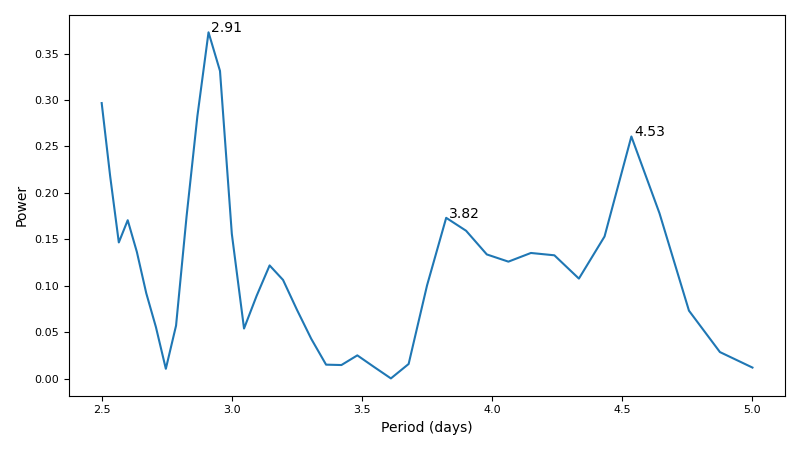
\includegraphics[scale=0.40]{REM/images/remcomb2022pgram.png} \\
\vspace{-.5cm}
\end{center}   
\caption{This shows part of the periodogram derived by starting from the
same data as in Fig. \ref{fig:rossallcurve} pertaining
to 2022 (up to 23 March), but calculating the ratio of the flux to
the sum of that from the 4 brightest stars common to all of the
images again restricting the display to 2.5 to 5 days.}\protect\label{fig:rosscombpgram}
\end{figure}

There is a suggestion of a longer period in Fig. \ref{fig:rossallcurve} which is
not observed in light curve plots for other objects, and Fig.
\ref{fig:rosslongperiod} shows a periodogram for periods between 500 and 2,000
days.

\begin{figure}[!htbp]
\begin{center}
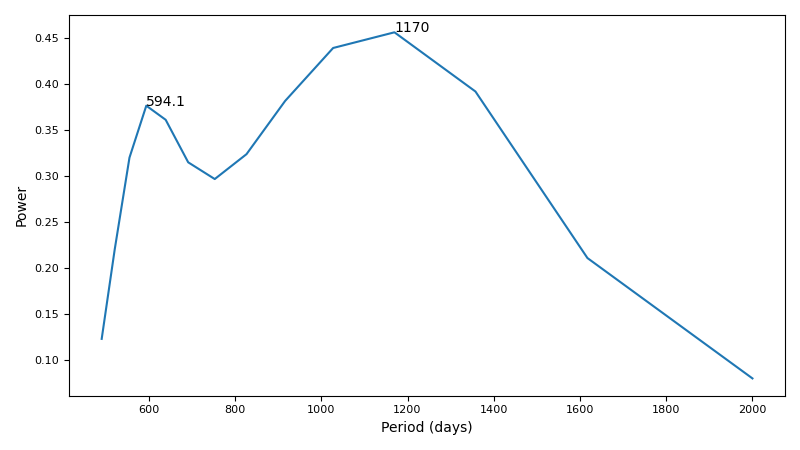
\includegraphics[scale=0.40]{REM/images/rosslongperiod.png} \\
\vspace{-.5cm}
\end{center}   
\caption{This shows the periodogram taken
over the whole of the data (as shown in Fig.
\ref{fig:rossallcurve}) showing peaks in the
range of 500 to 2,000 days.}\protect\label{fig:rosslongperiod}
\end{figure}

There are insufficiently long periods recorded in the {\rem} observations or
other data for this periodicity to be explored further.}

\subsubsection{Specific conclusions as to the {\rem} images}
\protect\label{section:remconclusions}

\IfThesis{
An important step in improvement of the {\rem} image processing would be to
improve the handling of reference stars by a linear regression of the expected flux derived
from the published or empirically-computed magnitudes to the observed flux for
each of the reference stars involved.} 

There is further work to be done in improving and tuning the aperture selection
for each of the reference stars and removing those found to be excessively
variable, notwithstanding any lack of indication of variability from the
catalogues. It is not anticipated that this will have a significant effect on
the periodogram results.

It is also necessary to improve the calibration files by better eliminating
defective pixels from the images and refining the uncertainty on an individual
pixel basis. This is not anticipated to make a large difference either.

However, it does not seem to be possible to improve the performance of the
{\rem} image processing significantly, to be confident of calculating rather
than merely confirming the figure derived from other methods.
It may well be that refinements to the calculations, especially with the
reference star classification of which over 600 were considered for \ross, may
yield better results, It should also be noted that {\ross} is on average nearly
70 times brighter in the images than the other objects. The uncertainty for the
{\ross} observations is approximately 0.27\% in the images, but that for the
other objects averages out at approximately 13\% due to the lack of contrast
between the objects and the sky level.

There might be scope for improvements by increasing the exposure times for the
images taken by the {\rem} telescope. This could be conveniently doubled without
risking saturation on the most useful filter images.
